\documentclass[letterpaper, 12pt]{report}
\usepackage[utf8]{inputenc}
\usepackage{amsmath,amssymb,amsthm}
\usepackage[spanish]{babel}
\usepackage{graphicx}
\usepackage{caption}
\usepackage{subcaption}
\usepackage{xcolor}
\usepackage{titlesec}
\usepackage{lmodern}
\usepackage{fancyhdr}
\usepackage{geometry}
\setlength{\headheight}{24.01996pt}
\addtolength{\topmargin}{-12.01996pt}

% Definir colores personalizados
\definecolor{primary}{RGB}{25,55,95}
\definecolor{secondary}{RGB}{200,35,45}

% Configurar márgenes
\geometry{
    left=3cm,
    right=2.5cm,
    top=3cm,
    bottom=2.5cm
}

\newtheorem*{theorem*}{Teorema}

% Configurar estilo de títulos
\titleformat{\chapter}[display]
{\normalfont\Huge\bfseries\color{primary}}
{\chaptertitlename\ \thechapter}{20pt}{\Huge}

\titleformat{\section}
{\normalfont\Large\bfseries\color{primary}}
{\thesection}{1em}{}

% Configurar encabezado y pie de página
\pagestyle{fancy}
\fancyhf{}
\fancyhead[L]{\small\textcolor{primary}{\nouppercase{\leftmark}}}
\fancyfoot[C]{\textcolor{primary}{\thepage}}
\renewcommand{\headrulewidth}{0.4pt}
\renewcommand{\headrule}{\hbox to\headwidth{\color{primary}\leaders\hrule height \headrulewidth\hfill}}

% Portada personalizada
\newcommand*{\customtitlepage}{
    \begin{titlepage}
        \begin{center}
            \vspace*{1cm}
            
            
            {\LARGE \textbf{UNIVERSIDAD DE LA HABANA}}\\
            \vspace{0.5cm}
            {\Large Facultad de Matem\'atica y Computaci\'on}\\
            

            
\includegraphics[scale=0.5]{images/logo.png}
            
            \vspace{1cm}
            
            
            \rule{\textwidth}{1.5pt}\\
            \vspace{0.5cm}
            {\LARGE \textcolor{primary}{\textbf{PROYECTO FINAL}}}\\
            {\LARGE \textcolor{primary}{\textbf{DISE\~NO Y AN\'ALISIS DE ALGORITMOS}}}
            \vspace{0.5cm}
            \rule{\textwidth}{1.5pt}
            
            \vspace{2cm}
            
            {\Large \textbf{Diseño Computacional de Prote\'inas}}\\
            \vspace{1cm}
            
            {\Large \textbf{Autor:} Lidier Robaina Caraballo \\
            \vspace{0.5cm}
            {\Large \textbf{Grupo:} C-411 }\\
            \vspace{1.5cm}
            
            {\Large \today}
            }
        \end{center}
    \end{titlepage}
}

\begin{document}

\customtitlepage

% Índice
\tableofcontents
\thispagestyle{empty}
\cleardoublepage

% Contenido principal
\setcounter{page}{1}

\chapter{Introducción}

La bioinform\'atica emerge como un campo revolucionario en la intersección entre la biología, la química y la ciencia de la computación, ofreciendo herramientas innovadoras para abordar desafíos científicos y tecnológicos de alto impacto. Las proteínas, como máquinas moleculares esenciales para la vida, desempeñan roles críticos en procesos biológicos, aplicaciones médicas (como el desarrollo de fármacos y terapias) y soluciones industriales (como biocatalizadores y materiales biodegradables). Sin embargo, el diseño tradicional de proteínas, basado en métodos experimentales de ensayo y error, resulta costoso, lento y limitado en complejidad. Aquí es donde los algoritmos computacionales se convierten en un aliado indispensable: permiten modelar, predecir y optimizar estructuras proteicas con precisión, acelerando el descubrimiento de soluciones biológicas personalizadas.  \\

La \textbf{motivación} de este proyecto radica en dos pilares fundamentales. Primero, la necesidad de explorar estrategias algorítmicas eficientes para resolver problemas NP-duros asociados al diseño de proteínas, como el plegamiento tridimensional y la estabilidad termodinámica. Segundo, la oportunidad de contribuir al avance de áreas como la medicina personalizada, la bioingeniería y la sostenibilidad ambiental, donde proteínas diseñadas a la medida podrían transformar paradigmas actuales. \\

Los \textbf{objetivos} del proyecto se centran en:
\begin{itemize}
    \item[1.] Modelar el problema de diseño de proteínas desde una perspectiva algorítmica, identy pueden realizar ificando sus componentes críticos (espacio de búsqueda, funciones de energía, restricciones biológicas).  
    \item[2.] Implementar y comparar algoritmos que aborden el diseño de secuencias, evaluando su eficiencia (tiempo y espacio) y efectividad (precisión y estabilidad de las soluciones).  
    \item[3.] Analizar limitaciones y ventajas de enfoques clásicos frente a métodos modernos basados en aprendizaje automático.  
\end{itemize}



\chapter{Definici\'on del Problema}

\section{Marco Te\'orico}

Las proteínas son macromol\'eculas esenciales para la vida dado que est\'an involucradas en casi todas las funciones estructurales,
catal\'iticas, sensoriales y regulatorias de los organismos. Est\'an formadas por una secuencia de compuestos org\'anicos llamadas aminoácidos,
y su función está determinada fundamentalmente por la estructura tridimensional que adopta la cadena de aminoácidos. \\  

El objetivo del diseño de proteínas es encontrar, dentro de una colección de proteínas, la que m\'as probabilidades tiene de ajustarse a una función.
Puesto que existen veinte aminoácidos posibles para cada posición en una secuencia proteica, y cada uno de ellos admite diversas variantes estructurales, 
la cantidad de combinaciones factibles a evaluar supera las posibilidades de cualquier método experimental, incluso en el caso de secuencias muy cortas.


\subsection{Esqueleto}

Como ilustra la figura \ref{fig1}, los aminoácidos est\'an formado por un n\'ucleo com\'un (\'atomos de H, C, N y O) y una
cadena lateral (R) que es espec\'ifica para cada uno de los 20. En una proteína, los núcleos de los amino\'acidos están
enlazados en una secuencia que forma el \textit{esqueleto} de la proteína. \\



El esqueleto es relativamente r\'igido y define la estructura tridimensional de la proteína (figura \ref{fig2}), por tanto se asume
que la proteína resultante del diseño conservar\'a el plegamiento global de la estructura base elegida. Es decir,
se considera que el esqueleto de la proteína está fijo y es entrada del problema del diseño de proteínas. \\

\newpage

\begin{figure}[h!]
    \begin{center}
        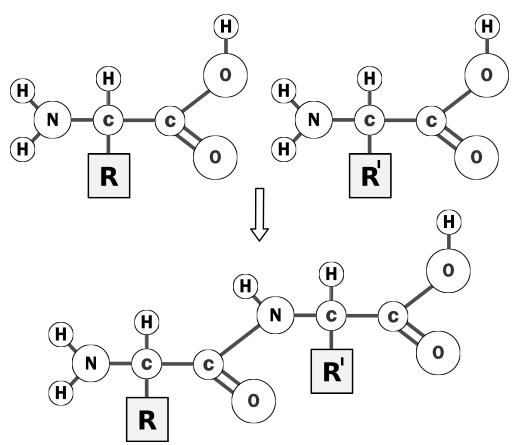
\includegraphics[scale=0.5]{images/dipeptido.png}
    \end{center}    
    \caption{Representaci\'on de c\'omo dos aminoácidos, con cadenas laterales espec\'ificas $R$ y $R'$, enlazan sus n\'ucleos para formar una cadena}
    \label{fig1}
\end{figure} 

\begin{figure}[h!]
    
    \begin{subfigure}[b]{0.49\textwidth}
        \begin{center}
            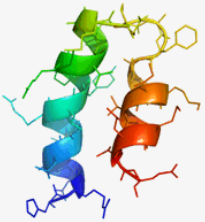
\includegraphics[scale=0.8]{images/protein.png} 
            \caption{Modelo con cadenas laterales}  
        \end{center}              
    \end{subfigure}    
    \begin{subfigure}[b]{0.49\textwidth}
        \begin{center}
            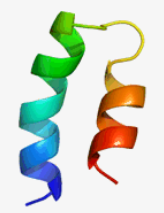
\includegraphics[scale=0.8]{images/backbone.png}  
            \caption{Esqueleto}  
        \end{center}             
    \end{subfigure}
    \caption{Modelo 3D de una proteína}
    \label{fig2}
\end{figure}









\subsection{Rot\'ameros}

Debido a la rotaci\'on alrededor de los enlaces simples, las cadenas laterales de los aminoácidos pueden adoptar distintas
conformaciones tridimensionales, que reciben el nombre de \textit{rotámeros}. Hay una cantidad 
infinita de rotámeros posibles, puesto que las moléculas pueden girar alrededor del eje de forma continua.
No obstante, suele ser suficiente considerar un conjunto discreto y representativo de rotámeros (figura \ref{fig3}),
el cual se puede determinar a través de un análisis estadístico de las conformaciones reales presentes en las 
bases de datos de estructuras de proteínas. \\

En el problema del diseño de proteínas, los rotámeros constituyen el espacio de b\'usqueda primario cuando el esqueleto está fijo.


\begin{figure}
    \begin{center}
        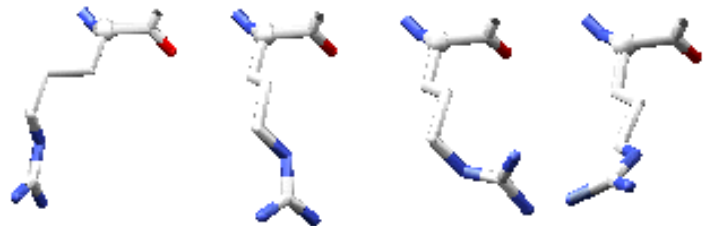
\includegraphics[scale=0.5]{images/rotameros.png}
    \end{center}    
    \caption{Rotámeros del aminoácido arginina: algunas posibles geometr\'ias de la cadena lateral}
    \label{fig3}
\end{figure} 

\subsection{Funciones de energ\'ia}

La estabilidad y la eficiencia funcional de una proteína están correlacionadas con su energía, por lo tanto, el objetivo
es encontrar la conformación que posea la energía total mínima. \\

La energía total de la proteína está dada por la energía del esqueleto, la energía de interacción entre los rotámeros y el esqueleto,
y la energía de interacción entre los diferentes rotámeros. Cuando el esqueleto está fijo, la minimización de la energía 
depende únicamente de la energía de interacción entre los rotámeros y entre estos y el esqueleto.
Sean $i_r$ el rotámero en la posición $i$, $E(i_r)$ la energía de interacción entre el rotámero $i$ y el esqueleto, 
y $E(i_r , j_{r'})$ la energía de interacción entre los rotámeros $r$ en la posición $i$ y $r'$ en la posición $j$, la fórmula a minimizar se convierte en

\[E = \sum_i E(i_r) + \sum_i \sum_{j<i} E(i_r , j_{r'})  \]

%Los valores de energía normalmente se miden en kcal/mol y deben ser precomputados y almacenados en memoria.


\section{Modelaci\'on como problema de teor\'ia de grafos}
 
Una proteína con $k$ residuos puede ser representada por un grafo $k$-partito $G = (V,E)$, de forma tal que:
\begin{itemize}
    \item hay una partición $V_i$ por cada residuo $i$
    \item hay un vértice $v \in V_i$ por cada rotámero candidato del residuo $i$
    \item la arista $\langle u,v \rangle$ denota la interacción entre los rotámeros $u$ y $v$
    \item el vértice $v$ tiene un costo $c_v$ que es igual a la energía de interacción entre el rotámero $v$ y el esqueleto
    \item la arista $\langle u,v \rangle$ tiene un costo $c_{ \langle u,v \rangle }$ que es igual a la energía de interacción entre el rotámero $u$ y el rotámero $v$ \\
\end{itemize}

El problema del \textbf{Dise\~no Computacional de Proteínas (DCP)} se define como:

\begin{quote}
    Dado un grafo $k$-partito $G = (V,E)$, $V = V_1 \cup V_2 \cup ... \cup V_k$, ponderado en vértices y aristas, hallar la asignaci\'on $a: [k] \rightarrow V$ con $a(i) \in V_i$, tal que 
    el costo 
    \[\sum_i c_{a(i)} + \sum_i \sum_{j<i} c_{ \langle a(i),a(j) \rangle }  \]
    del grafo inducido por el conjunto de vértices $ \lbrace a(i) \rbrace $ sea m\'inimo.
\end{quote}


\chapter{An\'alisis de complejidad}


Para demostrar que \textbf{DCP} es un problema \textbf{NP-Hard}, se realiza una reducción desde el \textbf{problema de Clique}:

\section{DCP $\in$ NP-Hard}

\subsection{Reducción Clique $\propto$ DCP}

Sea $ G = (V, E) $ un grafo no dirigido y $ k $ un entero (instancia del problema de Clique). Se construye un grafo n-partito $ G' $ para el problema de diseño de proteínas como sigue:

\begin{itemize}
    \item[1.] Particiones de $ G' $
    \begin{itemize}
        \item Cada vértice $ v_i \in V $ corresponde a una partición $ V_i $ en $ G' $.  
        \item Cada partición $ P_i $ tiene dos vértices:  
        \begin{itemize}
            \item $ a_i $ (representa "incluir $ v_i $ en el clique"), con peso 0. 
            \item $ b_i $ (representa "excluir $ v_i $"), con peso 1.  
        \end{itemize}
    \end{itemize}
    \item[2.] Aristas en $ G' $
    \begin{itemize}
        \item Para cada par de particiones $ V_i, V_j $ ($ i \neq j $): 
        \begin{itemize}
            \item Si $ \langle v_i, v_j \rangle \in E $, la arista $ \langle a_i, a_j \rangle $ tiene peso 0.  
            \item Si $ \langle v_i, v_j \rangle \notin E $, la arista $ \langle a_i, a_j \rangle $ tiene peso 1.  
        \end{itemize}
        \item Todas las aristas que involucran algún $ b_i $ tienen peso $ 0 $.  
    \end{itemize}    
\end{itemize}

% 1. **Particiones de $$ G' $$**:  
%    - Cada vértice $$ v_i \in V $$ corresponde a una partición $$ P_i $$ en $$ G' $$.  
%    - Cada partición $$ P_i $$ tiene dos vértices:  
%      - $$ a_i $$ (representa "incluir $$ v_i $$ en la clique"), con peso $$ 0 $$.  
%      - $$ b_i $$ (representa "excluir $$ v_i $$"), con peso $$ M $$ ($$ M \gg 0 $$).  

% 2. **Pesos de aristas en $$ G' $$**:  
%    - Para cada par de particiones $$ P_i, P_j $$ ($$ i \neq j $$):  
%      - Si $$ (v_i, v_j) \in E $$ en $$ G $$, la arista $$ (a_i, a_j) $$ tiene peso $$ 0 $$.  
%      - Si $$ (v_i, v_j) \notin E $$, la arista $$ (a_i, a_j) $$ tiene peso $$ M $$.  
%    - Todas las aristas que involucran algún $$ b_i $$ tienen peso $$ 0 $$.  

% ---

\subsection{Equivalencia de soluciones}

\begin{theorem*}
    $G$ tiene un clique de tamaño $k$ si y solo si $G'$ tiene un subgrafo inducido de peso menor o igual que 0.
\end{theorem*}

\noindent
\textbf{Demostración} \\


($\Rightarrow$) \\


Seleccionando los vértices $ a_i $ correspondientes a los $ k $ nodos del clique en $ G $, el subgrafo inducido en $ G' $ cumple que:  

\begin{itemize}
    \item Los vértices $ a_i $ tienen peso 0.  
    \item Las aristas entre ellos tienen peso 0 (porque forman un clique en $ G $).  
\end{itemize}

Por tanto, el peso total es de 0. \\

($\Leftarrow$) \\ 
 
\begin{itemize}
    \item Todos los vértices del subgrafo deben ser $ a_i $ (ya que cualquier $ b_i $ añadiría peso).
    \item Las aristas entre estos $ a_i $ deben tener peso 0, lo que implica que $ \langle v_i, v_j \rangle \in E $ para todo par.      
\end{itemize}

Esto corresponde a un clique de tamaño $ k $ en $ G $.  



% ---

% ### **Argumentos de complejidad**
% 1. **Construcción polinomial**:  
%    - $$ G' $$ tiene $$ 2|V| $$ vértices y $$ O(|V|^2) $$ aristas.  
%    - Los pesos se asignan en tiempo constante por arista.  

% 2. **Preservación de soluciones**:  
%    - Un algoritmo para el problema de diseño de proteínas resolvería Clique en tiempo polinomial, lo que es imposible a menos que $$ P = NP $$.  

% ---

% ### **Ejemplo ilustrativo**
% Considere $$ G $$ con vértices $$ \{1, 2, 3\} $$ y aristas $$ \{(1,2), (2,3)\} $$. Queremos ver si existe una clique de tamaño $$ k=2 $$.  
% - En $$ G' $$:  
%   - Particiones: $$ P_1 = \{a_1, b_1\}, P_2 = \{a_2, b_2\}, P_3 = \{a_3, b_3\} $$.  
%   - Aristas con peso $$ 0 $$: $$ (a_1, a_2) $$, $$ (a_2, a_3) $$.  
%   - Aristas con peso $$ M $$: $$ (a_1, a_3) $$.  
% - **Solución**: Seleccionar $$ a_1, a_2 $$ (clique en $$ G $$) → peso total = 0.  

% ---

% \section{Irreducibilidad de DCP}


% \chapter{Conclusiones}

% Al integrar fundamentos algorítmicos con desafíos biológicos, este proyecto no solo busca profundizar en el entendimiento teórico de problemas de optimización complejos, sino también demostrar cómo el diseño computacional puede catalizar innovaciones prácticas en bioingeniería.

\end{document}